\section{Approach and Solution Description}
\label{sec:solution-description}

As described in Sect.~\ref{sec:background}, CASCADE produces an inconsistency
verdict through a pipeline that combines
project extraction, filtering, LLM-based generation, repair, and test execution.
The final verdict alone does not reveal how much time or how many LLM resources
were required to reach it, nor where failures occurred along the way. Our
solution, implemented in our CASCADE fork,\footnote{\url{https://github.com/alexshristov/CASCADE}}
adds a structured measurement layer to this workflow. The layer
observes a run without participating in the inconsistency decision and produces
data that can be attributed to the responsible pipeline step. This changes the
benchmark from recording only whether CASCADE reached a result to also recording
how that result was produced and at what computational cost.

\subsection{Design Objectives and Constraints}
\label{sec:solution-objectives}

The main design challenge is that measurement is a cross-cutting concern.
Relevant observations originate at different depths of the pipeline: the
orchestration layer knows the run and its configuration, the analysis layer
knows the current sample and method, generators know the current task or repair
phase, and only the LLM caller sees response-level token usage. Similarly,
runtime is spent not only in LLM calls but also in Java project preparation,
Maven execution, and Docker setup. No single existing interface receives all of
this context.

We therefore define five objectives for the extension. First, observations must
be stored as structured data rather than as component-specific log messages.
Second, each observation should be attributable to its run and, where
available, to a sample, method, component, phase, and model. Third, adding a new
measurement must not require propagating a recorder and all context fields
through the complete call graph. Fourth, instrumentation must preserve
CASCADE's verdict, retry, and exception behavior. Finally, detailed observations
must remain available for later analyses, while common totals should be directly
accessible for model comparisons.

These objectives are subject to two practical constraints. A run may terminate
before normal completion, so partial measurements must remain useful. In
addition, CASCADE constructs interchangeable components from its configuration;
the measurement mechanism should preserve this extensibility instead of tying
the pipeline to one experiment-specific output routine.

\subsection{Run-Scoped Measurement Architecture}
\label{sec:solution-architecture}

The proposed architecture separates four responsibilities, as shown in
Fig.~\ref{fig:metrics-architecture}. A \emph{lifecycle owner} associates one
recorder with a pipeline invocation, activates it for the duration of the run,
and finalizes it regardless of whether the run succeeds. A small
\emph{instrumentation facade} offers operations for emitting an event, timing a
block, and temporarily adding attribution context. Pipeline components use this
facade without depending on the storage format. The \emph{event recorder}
enriches observations with run and context information, persists them, and
maintains aggregates. Finally, two \emph{measurement artifacts} serve different
uses: a detailed event stream supports auditing and new analyses, while a run
summary provides frequently used totals.

\begin{figure}[tb]
    \centering
    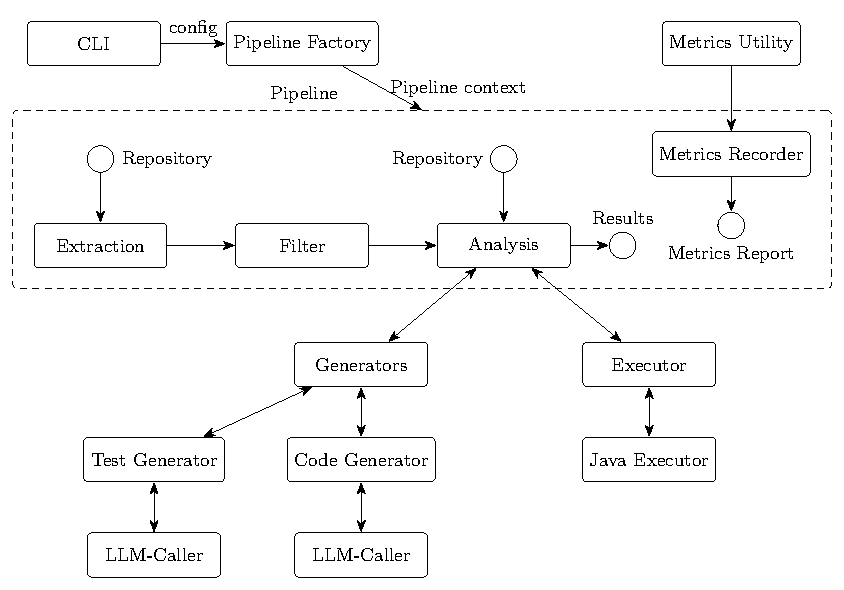
\includegraphics[width=\textwidth]{figures/metrics_architecture.pdf}
    \caption{Metrics data flow through CASCADE. Solid arrows show pipeline
    control flow; dashed arrows show observations sent through the shared
    instrumentation facade. The measurement layer observes the pipeline and
    does not modify its verdict flow.}
    \label{fig:metrics-architecture}
\end{figure}

The recorder is scoped to a run rather than being a permanent global sink.
Consequently, the same component can also be executed in isolation: when no
recorder is active, emitting an event has no effect. This avoids making metrics
a mandatory argument of every generator and executor interface. Recorder
construction remains configurable, following CASCADE's existing component
model, while instrumentation depends only on a minimal recorder contract.

Context is introduced progressively. The analysis scope contributes sample and
method identifiers, the generation scope adds its component and task, and a
nested generation step refines the phase. Events inherit the active fields, and
an explicitly supplied field can override a contextual default. A low-level LLM
call can therefore be assigned to the correct sample and generation phase even
though its caller does not receive those values as parameters. This approach
avoids both invasive parameter propagation and independent file-writing logic
in every component.

\subsection{Event and Context Model}
\label{sec:solution-event-model}

An event is a timestamped observation associated with a unique run identifier.
The design distinguishes three categories:

\paragraph{Timing events.}
These record the elapsed wall-clock time and success state of a bounded
operation, such as extraction, generation, repair, or test execution.
\paragraph{LLM-call events.}
These describe every invocation attempt, including the model and provider
endpoint, attempt number, elapsed time, finish state, normalized token usage,
and any failure information.
\paragraph{Semantic events.}
These record facts that are not durations, for example the number of extracted
or filtered samples, a skipped analysis, a per-method verdict, or completion of
a run.

For example, an LLM-call event may state that a successful call belongs to
sample~17, was issued by the test generator during its compilation-check phase,
used a particular model, consumed 2,400 input and 510 output tokens, and took
12.4 seconds. This single record contains the local response data and the
inherited pipeline context required to compare it with calls from other samples
and phases.

Durations are measured with a monotonic timer so that wall-clock adjustments do
not distort elapsed time. Failed attempts are recorded as well as successful
ones; otherwise a model that causes retries would appear artificially cheap.
Because OpenAI-compatible providers expose either prompt/completion or
input/output token fields, both forms are normalized to input, output, and total
tokens. If a provider supplies no usage metadata, the recorder does not infer
usage from the prompt. Monetary cost is likewise left to later analysis because
prices vary by provider and date, and locally hosted models have no meaningful
per-token API price.

\subsection{Persistence, Aggregation, and Failure Semantics}
\label{sec:solution-persistence}

The measurement layer deliberately produces two representations. Each complete
event is appended immediately to a JSON Lines stream. This stream is the source
of truth: it preserves event-level detail, can be processed by future analysis
scripts, and retains observations written before an interrupted run. In
parallel, the recorder folds every event into in-memory aggregates. At the end
of the run it writes a compact JSON summary containing event and failure counts,
timing totals, LLM usage grouped by model, component, and phase, and per-sample
statistics. A configuration snapshot and the run identifier link these
aggregates to the executed setup.

The summary is a convenience artifact rather than an independent measurement.
Keeping the raw stream avoids rerunning expensive experiments when an additional
grouping is needed, whereas the summary avoids repeatedly scanning all events
for common comparisons. Incremental aggregation also means that finalization
does not need to read the event file again.

Instrumentation follows best-effort failure semantics. A timed operation emits
its elapsed time and success state on both normal and exceptional exits, but an
exception from the observed operation is never suppressed. Run completion and
summary writing are attempted on the finalization path even after such an
exception. Conversely, failure to write a metrics event is reported and counted
but does not replace CASCADE's result or terminate its analysis. This preserves
the original tool behavior, although experiment processing must check metrics
completeness before treating a run as a valid observation.

\subsection{Design Decisions and Alternatives}
\label{sec:solution-decisions}

Table~\ref{tab:design-decisions} summarizes the principal decisions and the
alternatives rejected during the design. Together, they keep instrumentation
small enough to apply across the existing pipeline while retaining the detail
needed for reproducible evaluation.

\begin{table}[tb]
    \centering
    \caption{Main design decisions for the Metrics Recorder.}
    \label{tab:design-decisions}
    \small
    \begin{tabular}{@{}p{0.21\textwidth}p{0.32\textwidth}p{0.35\textwidth}@{}}
        \toprule
        \raggedright Decision & \raggedright Rationale & \raggedright Alternative considered \tabularnewline
        \midrule
        \raggedright Run-scoped context
            & \raggedright Attributes nested events with limited coupling
            & \raggedright Pass recorder and context through the call graph \tabularnewline
        \raggedright Structured events
            & \raggedright Enables consistent machine aggregation
            & \raggedright Extend free-form logs in each component \tabularnewline
        \raggedright Append-only event stream
            & \raggedright Retains detailed and partial data locally
            & \raggedright Keep data only in memory or use remote telemetry \tabularnewline
        \raggedright Events plus summary
            & \raggedright Supports auditability and efficient queries
            & \raggedright Store only aggregates or always rebuild totals \tabularnewline
        \raggedright Configurable recorder
            & \raggedright Preserves CASCADE's extensible model
            & \raggedright Hard-code one pipeline-wide file writer \tabularnewline
        \raggedright Best-effort writes
            & \raggedright Preserves analysis behavior if output fails
            & \raggedright Fail the pipeline when metrics output fails \tabularnewline
        \raggedright Deferred monetary cost
            & \raggedright Avoids provider- and time-dependent assumptions
            & \raggedright Embed a fixed model-pricing table \tabularnewline
        \bottomrule
    \end{tabular}
\end{table}

The design has explicit tradeoffs. Context-local state avoids widespread API
changes but assumes CASCADE's current, predominantly synchronous execution
model; concurrent execution would require controlled context propagation and
coordinated output writes. Local files improve inspection after a crash and do
not require observability infrastructure, but they do not provide distributed
real-time monitoring. Immediate event writes improve survivability at the cost
of additional I/O. Finally, best-effort recording protects the analysis but
requires downstream completeness checks.

\subsection{Analytical Capabilities and Scope}
\label{sec:solution-capabilities}

The resulting data model supports comparisons of total and per-phase runtime,
successful and failed LLM attempts, input and output token usage, generation and
repair activity, and Java/Docker execution overhead. These measurements can be
grouped by run, model, component, phase, or sample and related to the final
classification outcome. Sect.~\ref{sec:evaluation} defines how they are used
for the model comparison; the concrete integration points and artifacts are
described in Sect.~\ref{sec:implementation}.

The Metrics Recorder observes rather than optimizes CASCADE. It neither improves
inconsistency detection by itself nor makes stochastic LLM output deterministic.
It also does not replace the existing result artifacts or the quality metrics
derived from them. Instead, it supplies the missing measurement basis needed to
evaluate detection quality together with the resources and failures involved in
obtaining it.

\sectioncontributors{Bruno Vincent Hemoura, Alexander Hristov, and Caspar Moritz Klein.}
